%!TEX root = Report.tex

% Overvej at kalde dette afsnit "Experimentation" eller "Testing"
% 
% vis hvornår det virker og hvornår det ikke virker. 
% Se at det virker når vi regnede med at det virkede.
% 
% Hvad tester vi?
% Hvordan tester vi det?
% Virkede det efter hensigten?
% Hvorfor/hvorfor ikke?
% Er der nok testing?
% Hvordan kan man lave mere testing?
% Er der andre måder vi kunne have testet på? (fordele og ulemper ved det)

\subsection{Testing the tracking software with real ants}

Having solved the problem of finding an ant on a single image and integrated our software with the XY-plotter and camera, this section focus on testing how the integrated solution works with a video feed of an ant running arond in a controlled environment.\\

The test were performed in a ordinary office environment, with the plotter placed on a table. The room were only litten by daylight, and we used the setup explained in section (REF HANDLING ANTS), with a petridish filled with ground material surround by water, as can be seen in Figure (INSERT FIGURE WITH IMAGE OF SETUP). According to our experimentation in (INSERT REF TO EXPERIMENTATION) we painted our ant with a white color to have the best possible color for tracking.\\

In the following we will show several results of running the software, both where the tracking works as intented, but also situations where the software does not work. We will end this section with a summary of the challenges presented by this real-time testing and suggest possible solutions to the problems and an overall evaluation of how the software together with the plotter an camera performs performs. We will also comment on the important observations done during testing.\\

We will begin by showing several images from the test where the software tracking works. Examples can be seen in Figure \ref{fig:ant_tracking}. We are showin both the final thresholded image, as well as the original image. For this test, following values were used $\alpha = 2.0$ and $T = 240$.\\

\begin{figure}
        \centering
        \begin{subfigure}[b]{0.35\textwidth}
                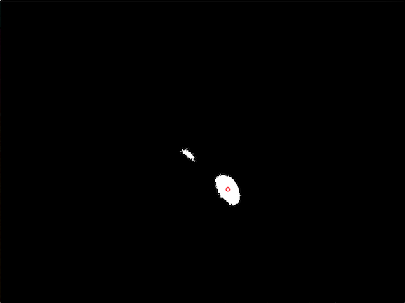
\includegraphics[scale = 0.3]{img/good1t}
                \caption{}
        \end{subfigure}
		\quad
        \begin{subfigure}[b]{0.35\textwidth}
                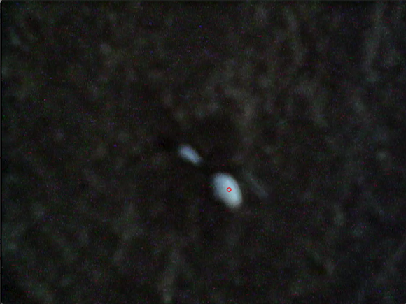
\includegraphics[scale = 0.3]{img/good1}
                \caption{}
        \end{subfigure} \hfill \\ \mbox{}\\
        \begin{subfigure}[b]{0.35\textwidth}
                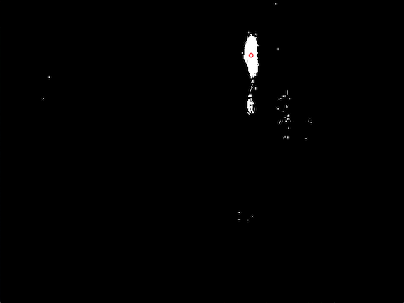
\includegraphics[scale = 0.3]{img/good2t}
                \caption{}
        \end{subfigure}
		\quad
        \begin{subfigure}[b]{0.35\textwidth}
                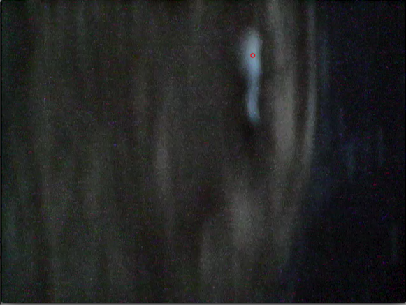
\includegraphics[scale = 0.3]{img/good2}
                \caption{}
        \end{subfigure}\hfill \\ \mbox{}\\
        \begin{subfigure}[b]{0.35\textwidth}
                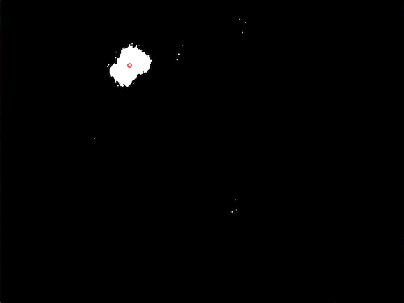
\includegraphics[scale = 0.3]{img/good3t}
                \caption{}
        \end{subfigure}
		\quad
        \begin{subfigure}[b]{0.35\textwidth}
                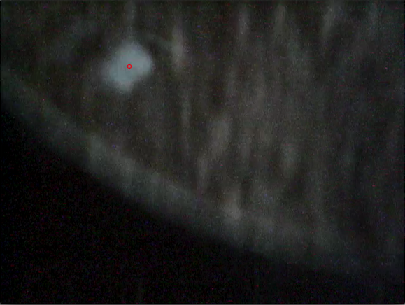
\includegraphics[scale = 0.3]{img/good3}
                \caption{}
        \end{subfigure}\\ \mbox{}\\
        \begin{subfigure}[b]{0.35\textwidth}
                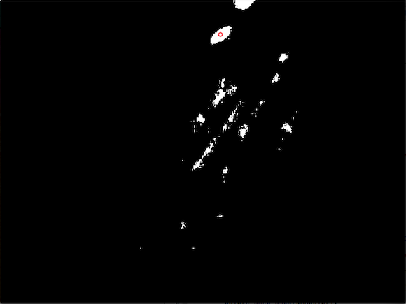
\includegraphics[scale = 0.3]{img/good4t}
                \caption{}
        \end{subfigure}
		\quad
        \begin{subfigure}[b]{0.35\textwidth}
                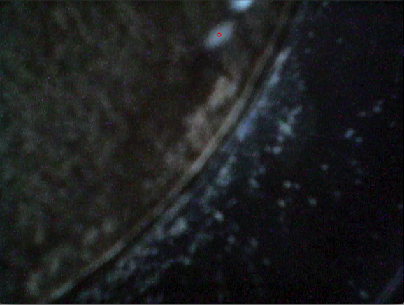
\includegraphics[scale = 0.3]{img/good4}
                \caption{}
        \end{subfigure}
		\caption{Examples of real-time ant tracking.}
		\label{fig:ant_tracking}
\end{figure}

We can see from the images in Figure \ref{fig:ant_tracking} that the software is able to handle different situations where a) the image is very blurry, b) there a noise in the thresholded images and c) where the ant is clearly visible. In general, we can say that it is possible to track the ant in situations where it is distinguishable from anything else in the image, or when it is the largest object present after image processing. However our tests also showed that at times we were unable to track the ant as shown in Figure \ref{fig:ant_fail}.\\

\begin{figure}
        \centering
        \begin{subfigure}[b]{0.35\textwidth}
                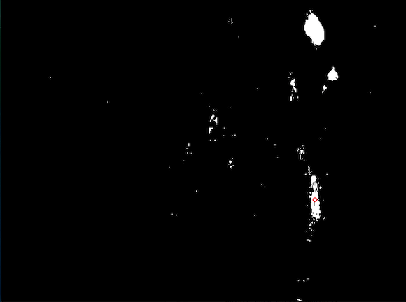
\includegraphics[scale = 0.3]{img/bad1t}
                \caption{}
        \end{subfigure}
		\quad
        \begin{subfigure}[b]{0.35\textwidth}
                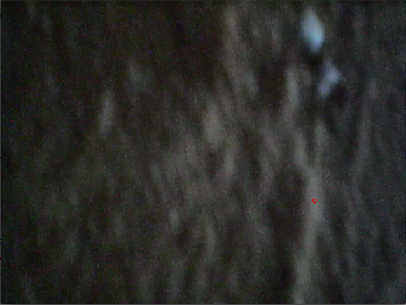
\includegraphics[scale = 0.3]{img/bad1}
                \caption{}
        \end{subfigure} \hfill \\ \mbox{}\\
        \begin{subfigure}[b]{0.35\textwidth}
                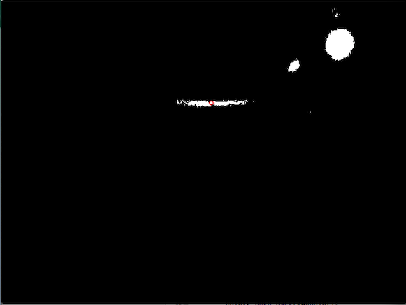
\includegraphics[scale = 0.3]{img/bad2t}
                \caption{}
        \end{subfigure}
		\quad
        \begin{subfigure}[b]{0.35\textwidth}
                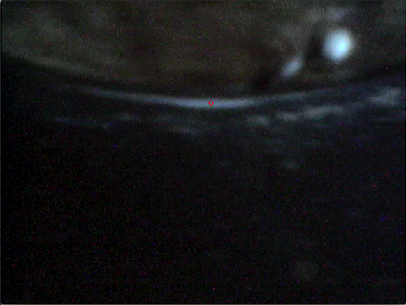
\includegraphics[scale = 0.3]{img/bad2}
                \caption{}
        \end{subfigure}\hfill \\ \mbox{}\\
        \begin{subfigure}[b]{0.35\textwidth}
                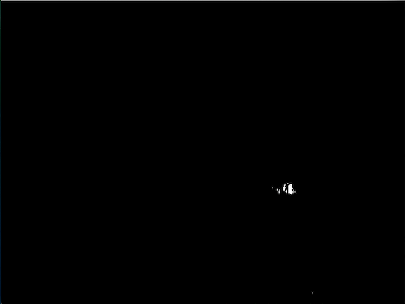
\includegraphics[scale = 0.3]{img/bad3t}
                \caption{}
        \end{subfigure}
		\quad
        \begin{subfigure}[b]{0.35\textwidth}
                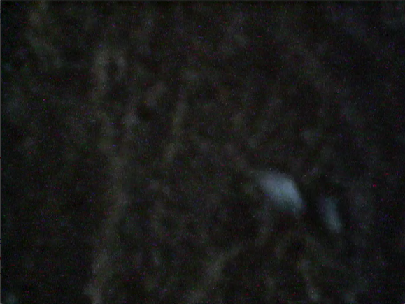
\includegraphics[scale = 0.3]{img/bad3}
                \caption{}
        \end{subfigure}\\ \mbox{}\\
        \begin{subfigure}[b]{0.35\textwidth}
                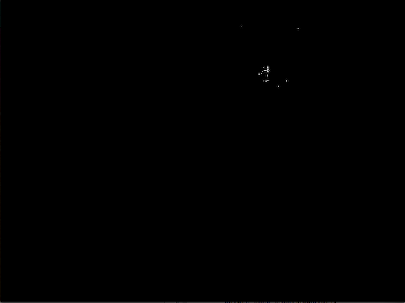
\includegraphics[scale = 0.3]{img/bad4t}
                \caption{}
        \end{subfigure}
		\quad
        \begin{subfigure}[b]{0.35\textwidth}
                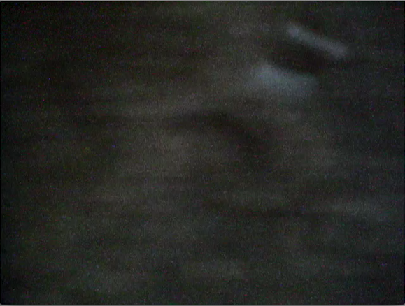
\includegraphics[scale = 0.3]{img/bad4}
                \caption{}
        \end{subfigure}
		\caption{Examples of tracking failues.}
		\label{fig:ant_fail}
\end{figure}

In image \emph{b} and \emph{d} in Figure \ref{fig:ant_fail}, the tracking fails because the ant is no longer the largest object in the thresholded images \emph{a} and \emph{c}. In image \emph{b} it is because the gound reflects too much light, and in image \emph{d} it is because the water reflects too much light. In image \emph{f} the problem arises because the images is too dark. Even with then given contrast, most of the white color does no make the threshold boundary, and the pixels that makes it past the thresold is considered noise by the blob detector. In image \emph{d} the image is simply too blurry (the ant is in the upper left corner), which makes both the ant and the white color "disappear" into the background.\\

\newpage